\begin{figure}[htbp]
\centering
\captionsetup{
  justification=raggedright,
  labelsep=none,
  singlelinecheck=false,
  labelformat=boldlabel,
}
\caption[Figure 10: \footnotesize ]{\footnotesize \textbf{: Agreement across base-learner predictions.} Pairwise correlation of the out-of-sample return predictions of the seven base learners (OLS, GLMNET, RF, XGB, NN1--NN3). Correlations are computed cross-sectionally within each month and then averaged over months, so they measure whether the models rank the same stocks alike rather than sharing a common time-series level. Lower correlations indicate more independent signals and hence more scope for the ensemble to add value.}
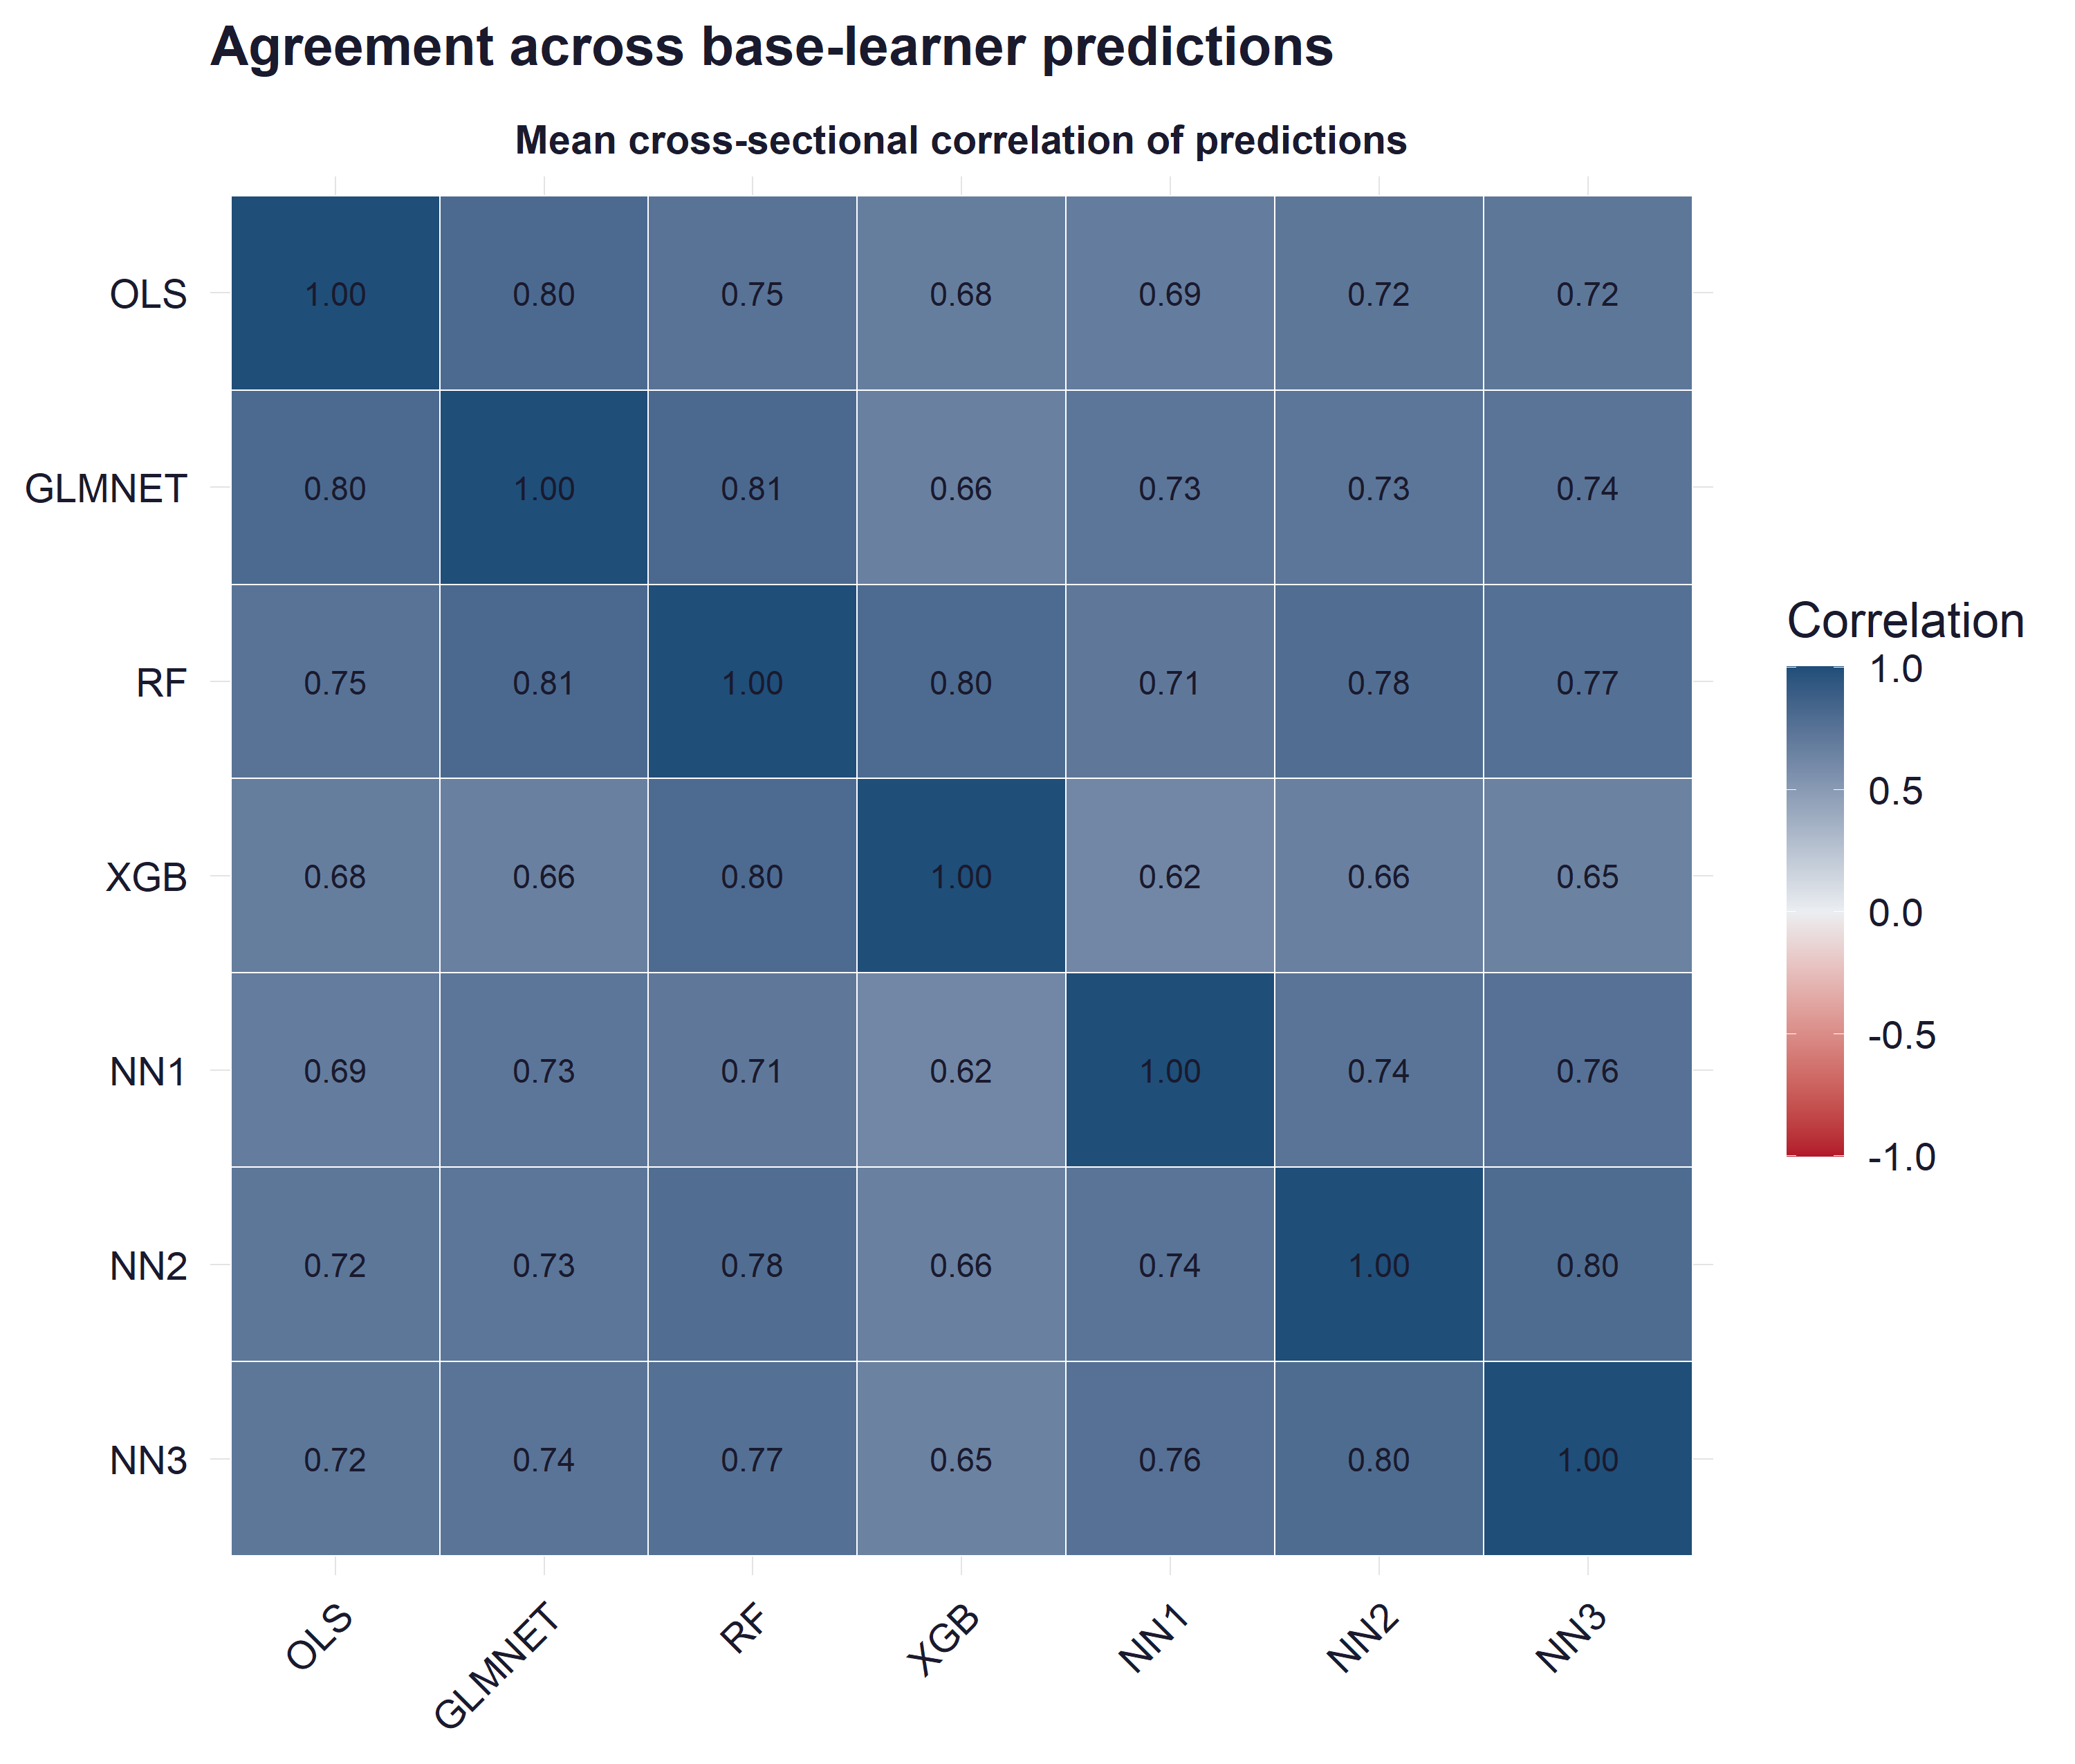
\includegraphics[width=\linewidth]{figures/correlogram_predictions.png}
\label{fig:corr_pred}
\end{figure}

\begin{figure}[htbp]
\centering
\captionsetup{
  justification=raggedright,
  labelsep=none,
  singlelinecheck=false,
  labelformat=boldlabel,
}
\caption[Figure 11: \footnotesize ]{\footnotesize \textbf{: Active return correlation: ML Ensemble portfolios vs human managers.} Monthly active return correlations (each series measured net of IBOV) among the eight ML Ensemble portfolio-construction schemes and the human-manager benchmarks FUNDS\_MEAN and FUNDS\_Q75. Active rather than raw returns are shown because the common market exposure of long-only portfolios mechanically pushes every raw-return pair toward one. All fund and IBOV returns are geometrically compounded 15th-to-15th to match the ML backtest. AVG\_FUND and AVG\_FUND\_Q75 are not return series: their entries average each portfolio's correlations with, respectively, all reliable funds and reliable top-quartile funds. Their diagonal entries average distinct within-cohort fund pairs and therefore are not equal to one. Lower ML-versus-fund correlations indicate greater diversification potential from combining machine and human portfolios.}
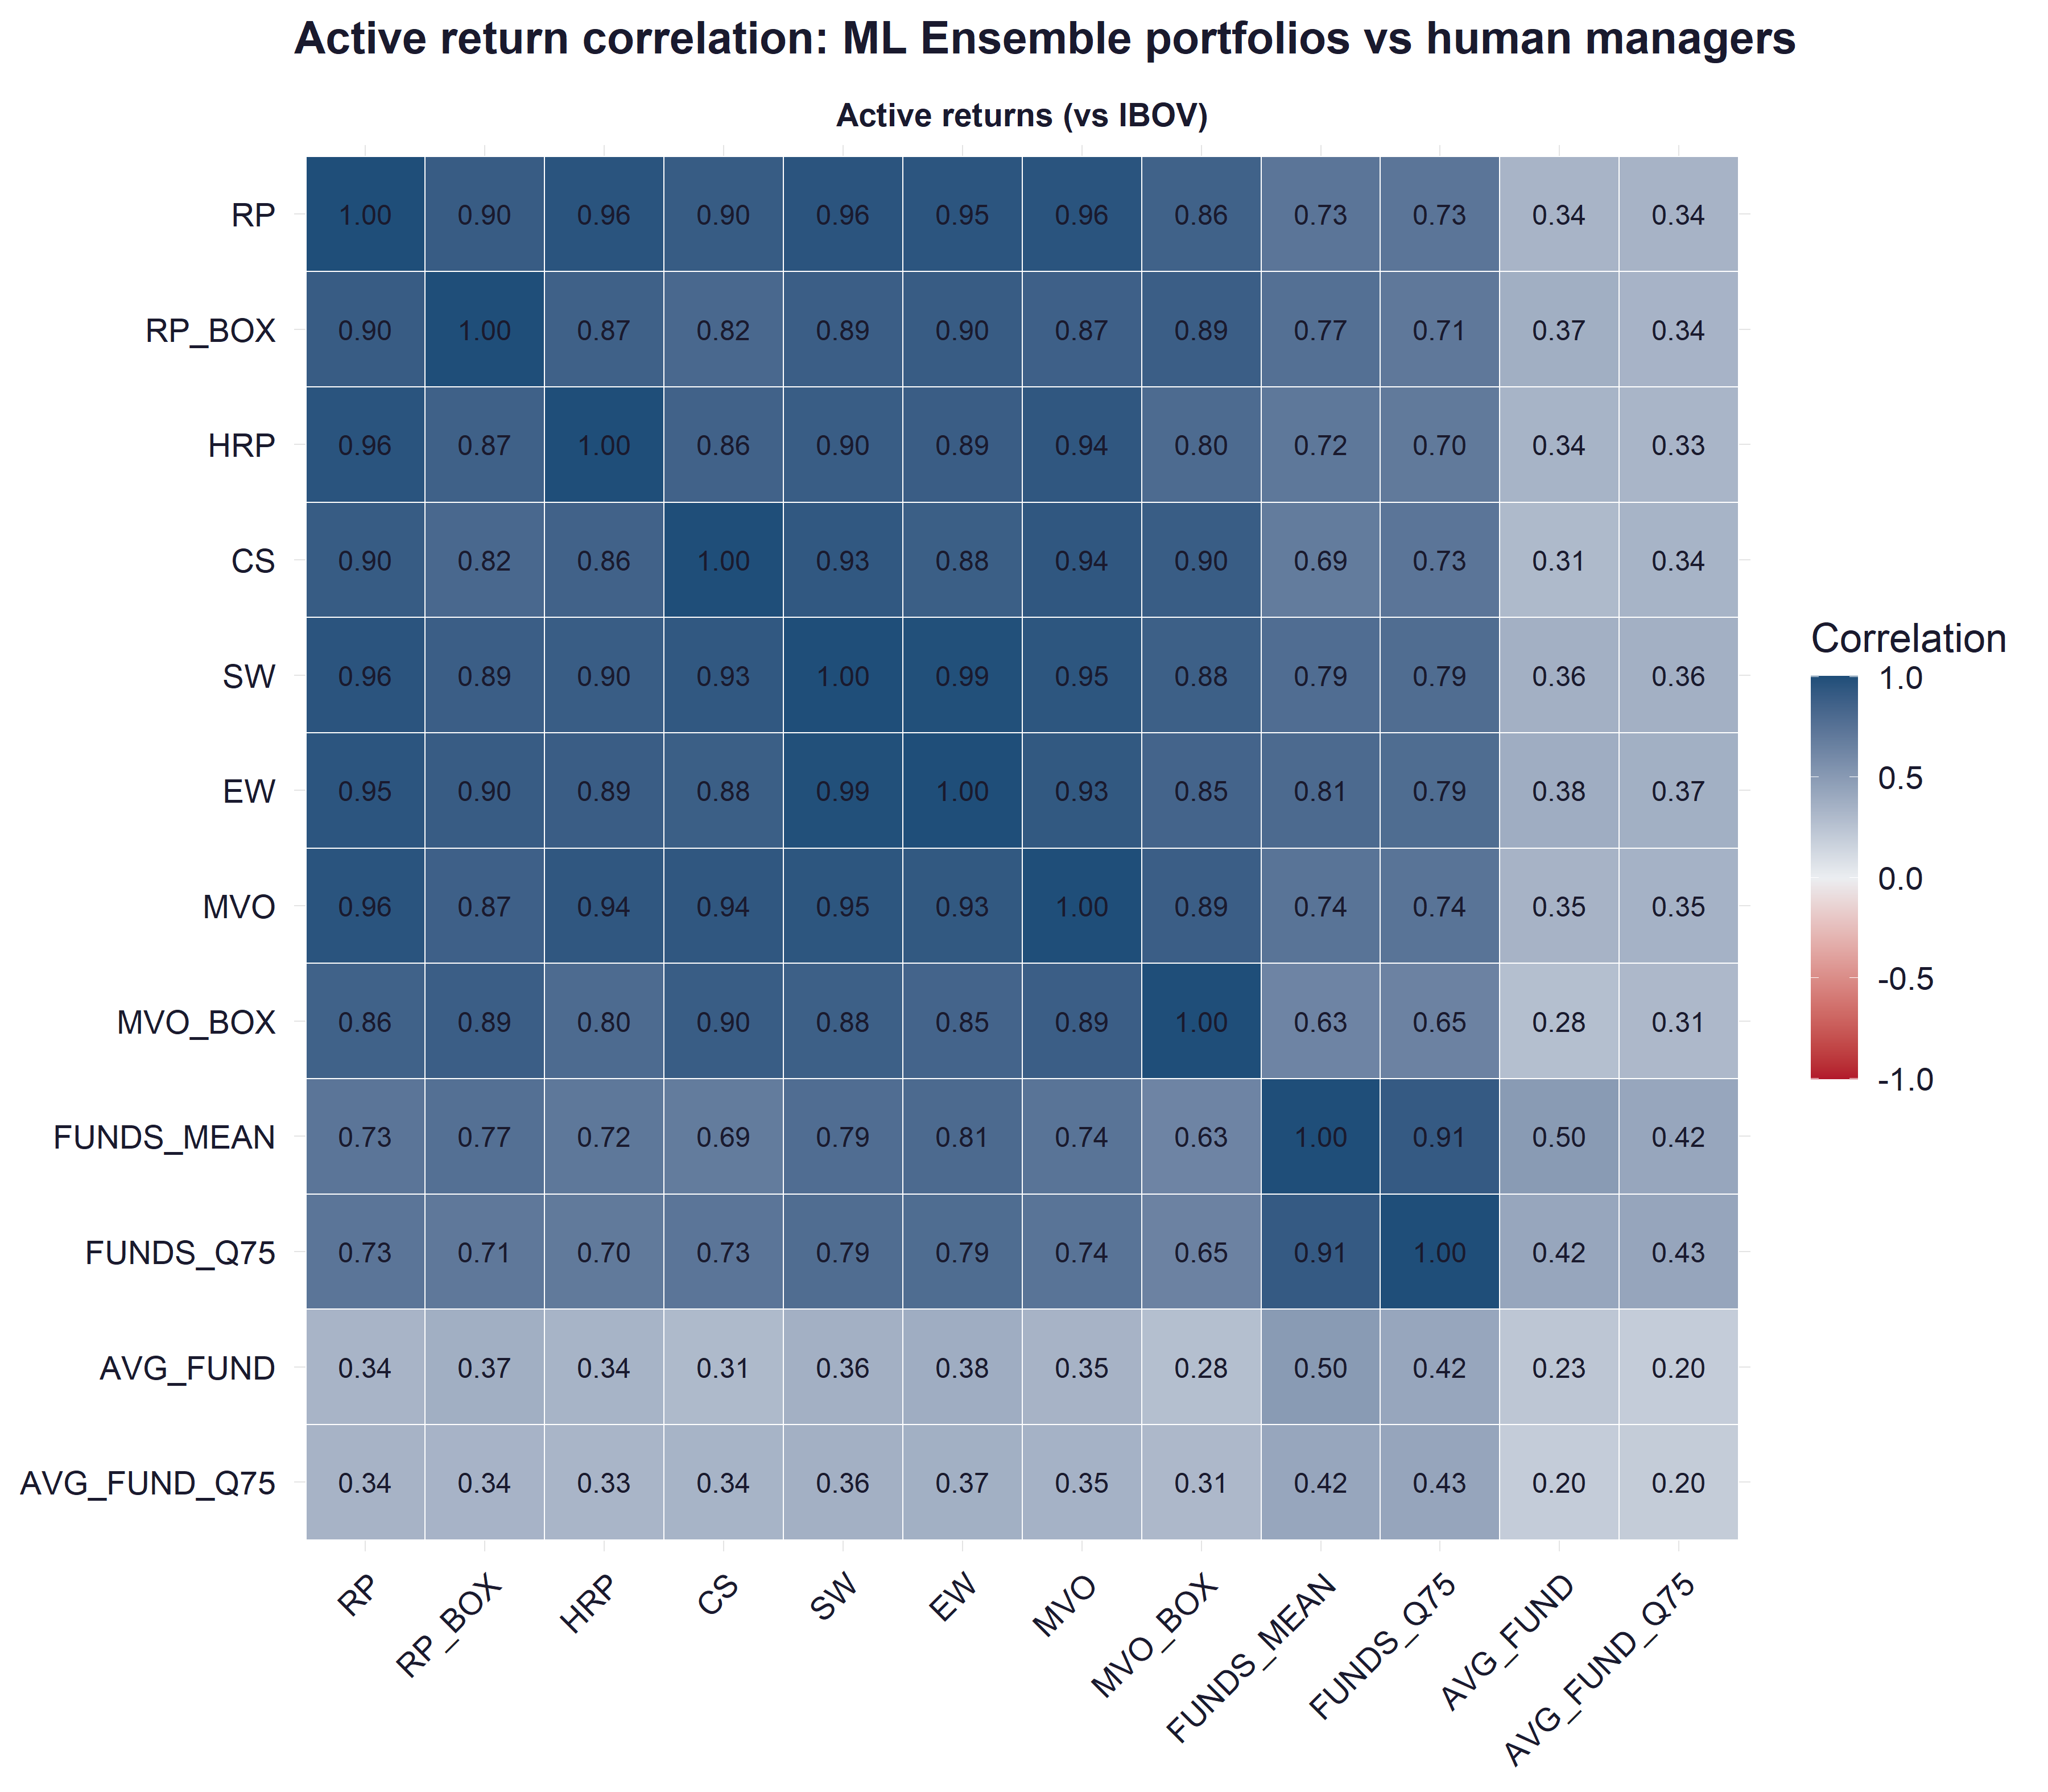
\includegraphics[width=\linewidth]{figures/correlogram_performance.png}
\label{fig:corr_perf}
\end{figure}
